\documentclass{beamer}

\usepackage[utf8]{inputenc}
\usepackage[spanish]{babel}

\xdefinecolor{lavanda}{rgb}{1,0.3,0.3}
\xdefinecolor{oliva}{cmyk}{0.64,0,0.95,0.4}
\xdefinecolor{minaranja}{rgb}{0.94,0.48,0.2}

\usetheme{Madrid}
\usecolortheme[named=lavanda]{structure}

\title[Computación Cuántica]{Introducción a la Computación Cuántica}
\author{Luis Aguirre \& Javier Pellejero}
\institute[UCM]{Universidad Complutense de Madrid\\ Facultad de Informática}


\newcommand{\base}[1]{|#1\rangle}
\newcommand{\lbase}[1]{\langle#1|}
\newcommand{\baseup}{\mid\uparrow\rangle}
\newcommand{\baseright}{\mid\rightarrow\rangle}
\newcommand{\baseupright}{\mid\nearrow\rangle}
\newcommand{\baseupleft}{\mid\nwarrow\rangle}

\begin{document}

\begin{frame}
	\titlepage
\end{frame}

\begin{frame}
\frametitle{Índice}
	\tableofcontents
\end{frame}

\section{Una primera aproximación mediante la polarización de fotones}

\begin{frame}
	\frametitle{Una aproximación mediante la polarización de fotones}
	Tenemos tres filtros de polarización de luz:
	\begin{itemize}
		\item \textbf{Filtro A:} de polarización horizontal $\rightarrow$.
		\item \textbf{Filtro B:} de polarización diagonal $\nearrow$.
		\item \textbf{Filtro C:} de polarización vertical $\uparrow$.
	\end{itemize}
	\begin{center}
	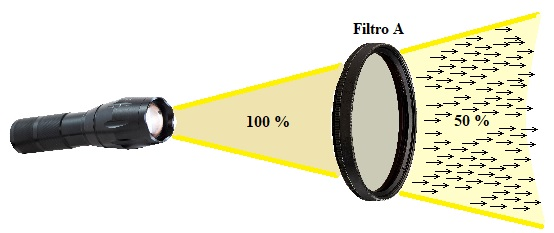
\includegraphics[scale=0.6]{imagenes/polarizacion1}\\
	Experimento 1.
	\end{center}
\end{frame}

\begin{frame}
	\frametitle{Una aproximación mediante la polarización de fotones}
	\begin{center}
	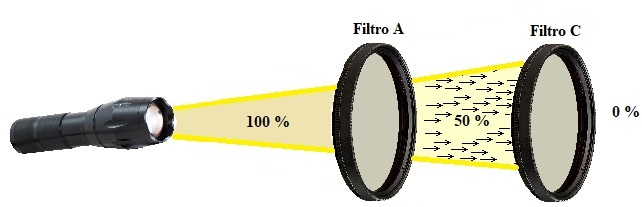
\includegraphics[scale=0.6]{imagenes/polarizacion2}\\
	Experimento 2.
	\end{center}		
\end{frame}

\begin{frame}
	\frametitle{Una aproximación mediante la polarización de fotones}
	\begin{center}
	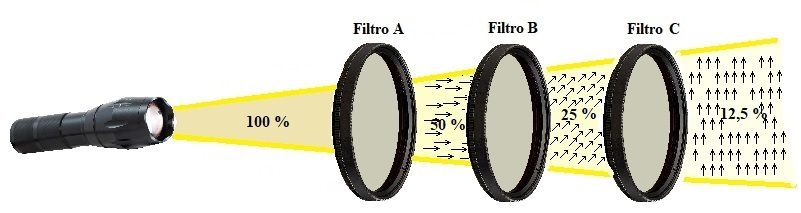
\includegraphics[scale=0.55]{imagenes/polarizacion3}\\
	Experimento 3.
	\end{center}
\end{frame}





\end{document}
